\documentclass[addpoints]{exam}
\usepackage[margin=0.75in]{geometry}
\usepackage{amsmath}
\usepackage{amssymb}
\usepackage{amsthm}
\usepackage{calc}
\usepackage{enumitem}
\usepackage{tikz}
\usepackage{float}
\usepackage{titling}
\usepackage{listings}
\usepackage{pdfpages}
\usepackage{setspace}
\usepackage{comment}
\usepackage{xcolor}
\usepackage{lmodern}
\pagestyle{headandfoot}

\pagestyle{headandfoot}
\runningheadrule
\runningfootrule
\runningheader{PHY 202}{}{\theauthor}
\runningfooter{}{Page \thepage\ of \numpages}{}
\firstpageheader{}{}{}

\boxedpoints
\printanswers

\newcommand\mbb[1]{\ensuremath{\mathbb{#1}}}
\renewcommand{\qedsymbol}{\ensuremath{\blacksquare}}

\title{PHY 202 - Quantum Mechanics - Assignment \# 5}
\author{Muhammad Meesum Ali Qazalbash - mq06861}

\begin{document}

\maketitle

\begin{questions}
    \question[15] Refer to the Question paper attached below.
    \begin{solution}
        \begin{enumerate}
            \item \begin{equation*}
                      \begin{aligned}
                          \left<\hat{p}\right>          & = \int_{-\infty}^{\infty} \psi^*(x)\hat{p}\psi(x) dx                                                                                                                                                                                  \\
                          \implies                      & = \int_{-\infty}^{\infty} \left(\frac{1}{\sqrt{2\pi}}\int_{-\infty}^{\infty}e^{-ik_1x}\tilde{\psi}^*(k_1)dk_1\right)\hat{p}\left(\frac{1}{\sqrt{2\pi}}\int_{-\infty}^{\infty}e^{ik_2x}\tilde{\psi}(k_2)dk_2\right) dx                 \\
                          \implies                      & = \frac{1}{2\pi}\int_{-\infty}^{\infty} \left(\int_{-\infty}^{\infty}e^{-ik_1x}\tilde{\psi}^*(k_1)dk_1\right)\left(-i\hslash \frac{\partial}{\partial x} \right)\left(\int_{-\infty}^{\infty}e^{ik_2x}\tilde{\psi}(k_2)dk_2\right) dx \\
                          \implies                      & = \frac{\hslash}{2\pi}\int_{-\infty}^{\infty} \left(\int_{-\infty}^{\infty}e^{-ik_1x}\tilde{\psi}^*(k_1)dk_1\right)\left(\int_{-\infty}^{\infty}k_2e^{ik_2x}\tilde{\psi}(k_2)dk_2\right) dx                                           \\
                          \implies                      & = \hslash\int_{-\infty}^{\infty} \int_{-\infty}^{\infty}\tilde{\psi}^*(k_1)\left(\frac{1}{2\pi}\int_{-\infty}^{\infty}e^{-i(k_1-k_2)x}dx\right)k_2 \tilde{\psi}(k_2) dk_1dk_2                                                         \\
                          \implies                      & = \hslash\int_{-\infty}^{\infty} \int_{-\infty}^{\infty}\tilde{\psi}^*(k_1)\delta(k_1-k_2)k_2 \tilde{\psi}(k_2) dk_1dk_2                                                                                                              \\
                          \implies                      & = \hslash\int_{-\infty}^{\infty} \left(\int_{-\infty}^{\infty}\tilde{\psi}^*(k_1)\delta(k_1-k_2)dk_1\right)k_2 \tilde{\psi}(k_2) dk_2                                                                                                 \\
                          \implies                      & = \hslash\int_{-\infty}^{\infty} k_2 \tilde{\psi}^*(k_2) \tilde{\psi}(k_2) dk_2                                                                                                                                                       \\
                          \implies \left<\hat{p}\right> & = \hslash\int_{-\infty}^{\infty} k \left|\tilde{\psi}(k)\right|^2 dk                                                                                                                                                                  \\
                      \end{aligned}
                  \end{equation*}
                  \pagebreak
            \item \begin{equation*}
                      \begin{aligned}
                          \left<\hat{p}^2\right>          & = \int_{-\infty}^{\infty} \psi^*(x)\hat{p}^2\psi(x) dx                                                                                                                                                                                  \\
                          \implies                        & = \int_{-\infty}^{\infty} \left(\frac{1}{\sqrt{2\pi}}\int_{-\infty}^{\infty}e^{-ik_1x}\tilde{\psi}^*(k_1)dk_1\right)\hat{p}^2\left(\frac{1}{\sqrt{2\pi}}\int_{-\infty}^{\infty}e^{ik_2x}\tilde{\psi}(k_2)dk_2\right) dx                 \\
                          \implies                        & = \frac{1}{2\pi}\int_{-\infty}^{\infty} \left(\int_{-\infty}^{\infty}e^{-ik_1x}\tilde{\psi}^*(k_1)dk_1\right)\left(-i\hslash \frac{\partial}{\partial x} \right)^2\left(\int_{-\infty}^{\infty}e^{ik_2x}\tilde{\psi}(k_2)dk_2\right) dx \\
                          \implies                        & = \frac{\hslash^2}{2\pi}\int_{-\infty}^{\infty} \left(\int_{-\infty}^{\infty}e^{-ik_1x}\tilde{\psi}^*(k_1)dk_1\right)\left(\int_{-\infty}^{\infty}k_2^2e^{ik_2x}\tilde{\psi}(k_2)dk_2\right) dx                                         \\
                          \implies                        & = \hslash^2\int_{-\infty}^{\infty} \int_{-\infty}^{\infty}\tilde{\psi}^*(k_1)\left(\frac{1}{2\pi}\int_{-\infty}^{\infty}e^{-i(k_1-k_2)x}dx\right)k_2^2 \tilde{\psi}(k_2) dk_1dk_2                                                       \\
                          \implies                        & = \hslash^2\int_{-\infty}^{\infty} \int_{-\infty}^{\infty}\tilde{\psi}^*(k_1)\delta(k_1-k_2)k_2^2 \tilde{\psi}(k_2) dk_1dk_2                                                                                                            \\
                          \implies                        & = \hslash^2\int_{-\infty}^{\infty} \left(\int_{-\infty}^{\infty}\tilde{\psi}^*(k_1)\delta(k_1-k_2)dk_1\right)k_2^2 \tilde{\psi}(k_2) dk_2                                                                                               \\
                          \implies                        & = \hslash^2\int_{-\infty}^{\infty} k_2^2 \tilde{\psi}^*(k_2) \tilde{\psi}(k_2) dk_2                                                                                                                                                     \\
                          \implies \left<\hat{p}^2\right> & = \hslash^2\int_{-\infty}^{\infty} k^2 \left|\tilde{\psi}(k)\right|^2 dk                                                                                                                                                                \\
                      \end{aligned}
                  \end{equation*}
            \item \begin{equation*}
                      \begin{aligned}
                          \left<f(\hat{p})\right>          & = \int_{-\infty}^{\infty} \psi^*(x)f(\hat{p})\psi(x) dx                                                                                                                                                                                                                    \\
                          \implies                         & = \int_{-\infty}^{\infty} \left(\frac{1}{\sqrt{2\pi}}\int_{-\infty}^{\infty}e^{-ik_1x}\tilde{\psi}^*(k_1)dk_1\right)f(\hat{p})\left(\frac{1}{\sqrt{2\pi}}\int_{-\infty}^{\infty}e^{ik_2x}\tilde{\psi}(k_2)dk_2\right) dx                                                   \\
                          \implies                         & = \int_{-\infty}^{\infty} \left(\frac{1}{\sqrt{2\pi}}\int_{-\infty}^{\infty}e^{-ik_1x}\tilde{\psi}^*(k_1)dk_1\right)\sum_{j\geq 0}\frac{f^{(j)}(0)}{j!}\hat{p}^j\left(\frac{1}{\sqrt{2\pi}}\int_{-\infty}^{\infty}e^{ik_2x}\tilde{\psi}(k_2)dk_2\right) dx                 \\
                          \implies                         & = \frac{1}{2\pi}\int_{-\infty}^{\infty} \left(\int_{-\infty}^{\infty}e^{-ik_1x}\tilde{\psi}^*(k_1)dk_1\right)\sum_{j\geq 0}\frac{f^{(j)}(0)}{j!}\left(-i\hslash \frac{\partial}{\partial x} \right)^j\left(\int_{-\infty}^{\infty}e^{ik_2x}\tilde{\psi}(k_2)dk_2\right) dx \\
                          \implies                         & = \frac{1}{2\pi}\int_{-\infty}^{\infty} \left(\int_{-\infty}^{\infty}e^{-ik_1x}\tilde{\psi}^*(k_1)dk_1\right)\sum_{j\geq 0}\frac{f^{(j)}(0)}{j!}(-i)^j\left(\int_{-\infty}^{\infty}i^j\hslash^jk_2^je^{ik_2x}\tilde{\psi}(k_2)dk_2\right) dx                               \\
                          \implies                         & = \frac{1}{2\pi}\int_{-\infty}^{\infty} \left(\int_{-\infty}^{\infty}e^{-ik_1x}\tilde{\psi}^*(k_1)dk_1\right)\left(\int_{-\infty}^{\infty}\sum_{j\geq 0}\frac{f^{(j)}(0)}{j!}(\hslash k_2)^je^{ik_2x}\tilde{\psi}(k_2)dk_2\right) dx                                       \\
                          \implies                         & = \frac{1}{2\pi}\int_{-\infty}^{\infty} \left(\int_{-\infty}^{\infty}e^{-ik_1x}\tilde{\psi}^*(k_1)dk_1\right)\left(\int_{-\infty}^{\infty}f(\hslash k_2)e^{ik_2x}\tilde{\psi}(k_2)dk_2\right) dx                                                                           \\
                          \implies                         & = \int_{-\infty}^{\infty} \int_{-\infty}^{\infty}\tilde{\psi}^*(k_1)\left(\frac{1}{2\pi}\int_{-\infty}^{\infty}e^{-i(k_1-k_2)x}dx\right)f(\hslash k_2) \tilde{\psi}(k_2) dk_1dk_2                                                                                          \\
                          \implies                         & = \int_{-\infty}^{\infty} \int_{-\infty}^{\infty}\tilde{\psi}^*(k_1)\delta(k_1-k_2)f(\hslash k_2) \tilde{\psi}(k_2) dk_1dk_2                                                                                                                                               \\
                          \implies                         & = \int_{-\infty}^{\infty} \left(\int_{-\infty}^{\infty}\tilde{\psi}^*(k_1)\delta(k_1-k_2)dk_1\right)f(\hslash k_2) \tilde{\psi}(k_2) dk_2                                                                                                                                  \\
                          \implies                         & = \int_{-\infty}^{\infty} f(\hslash k_2) \tilde{\psi}^*(k_2) \tilde{\psi}(k_2) dk_2                                                                                                                                                                                        \\
                          \implies \left<f(\hat{p})\right> & = \int_{-\infty}^{\infty} f(\hslash k) \left|\tilde{\psi}(k)\right|^2 dk                                                                                                                                                                                                   \\
                      \end{aligned}
                  \end{equation*}
        \end{enumerate}
    \end{solution}
    \pagebreak
    \question[15] Refer to the Question paper attached below.
    \begin{solution}
        \begin{enumerate}
            \item \(\psi_A\) would evolve with time as,
                  \[\psi_A(x,t) = \frac{1}{\sqrt{6}}\varphi_0(x)e^{-iE_0t/\hslash}+\frac{1}{\sqrt{3}}\varphi_1(x)e^{-iE_1t/\hslash}+\frac{1}{\sqrt{2}}\varphi_2(x)e^{-iE_2t/\hslash}\]
            \item It is given that,
                  \begin{equation*}
                      \begin{aligned}
                          E_n = \frac{(n+1)^2\pi^2}{mL^2} & \implies \forall n > 0, E_n = (n+1)^2E_0                                                                         \\
                          \left<\hat{E}\right>            & = \left(\frac{1}{\sqrt{6}}\right)^2E_0+\left(\frac{1}{\sqrt{3}}\right)^2E_1+\left(\frac{1}{\sqrt{2}}\right)^2E_2 \\
                          \left<\hat{E}\right>            & = \frac{1}{6}E_0+\frac{4}{3}E_0+\frac{9}{2}E_0                                                                   \\
                          \left<\hat{E}\right>            & = 6E_0
                      \end{aligned}
                  \end{equation*}
                  The Energy eign values do not change with time.
            \item We have,
                  \begin{equation*}
                      \begin{aligned}
                          \left<\hat{E}\right> & = 6E_0 \\
                          (n+1)^2E_0           & = 6E_0
                      \end{aligned}
                  \end{equation*}
                  But there exists no integer value of \(n\) such that \((n+1)^2\) is 6. Hence, the probability of measuring the energy equals to \(\left<\hat{E}\right>\) at time \(t=0\) and \(t=t_1\) is zero.
            \item The energy values which will be measured are \(E_0\) with probability of \(\frac{1}{6}\), \(E_1\) with probability of \(\frac{1}{3}\) and \(E_2\) with probability of \(\frac{1}{2}\). These probability are conserved which means they do not change with time.
            \item If \(E_2\) is measured at time \(t=t_1\) then for the time \(t>t_1\) the wave function will be,
                  \[\psi_A(x,t) = \varphi_2(x)e^{-iE_2t/\hslash}\]
                  This means all the states except the state with energy \(E_2\) will be zero. This means all other states have been collapsed.
            \item Let our new wave function be \(\psi_B\). For \(\psi_B\) to have same energies and probabilities, coeffiecents needs to be same. But for independence \(\psi_A\) must be orthogonal to \(\psi_B\), we would alter the sign of the wave function,
                  \[\psi_B(x,0)=\frac{1}{\sqrt{6}}\varphi_0(x)+\frac{1}{\sqrt{3}}\varphi_1(x)-\frac{1}{\sqrt{2}}\varphi_2(x)\]
            \item The new wave function will be,
                  \[\psi_C(x,0)=\sqrt{\frac{7}{4}}\varphi_0(x)+\frac{1}{\sqrt{2}}\varphi_1(x)+\frac{1}{\sqrt{4}}\varphi_2(x)\]
                  Verify that the new wave function has same total energy as \(\psi_A\).
                  \[\left<\hat{E}\right> = \frac{7}{4}E_0+\frac{4}{2}E_0+\frac{9}{4}E_0 = 6E_0\]
        \end{enumerate}
    \end{solution}

    \pagebreak
    \question[] Refer to the Question paper attached below.
    \begin{solution}
        Solving using time independent Schrodinger equation,
        \[\nabla^2\psi-\frac{2m}{\hslash^2}(V-E)\psi=0\]
        \[\frac{d^2\psi}{dx^2}-\frac{2m}{\hslash^2}(V-E)\psi=0\]
        For \(x>0\), we have,
        \[\frac{d^2\psi}{dx^2}+\frac{2m}{\hslash^2}E\psi=0\]
        Now let \(\displaystyle\frac{2mE}{\hslash^2}=\alpha^2\), then our equation becomes,
        \[\frac{d^2\psi}{dx^2}+\alpha^2\psi=0\]
        Therefore the solution to this ODE is,
        \[\psi(x)=A\sin(\alpha x)+B\cos(\alpha x)\]
        For \(x=0\implies\psi(x)=0\) as the potentail goes to infinite,
        \[0=A\sin(\alpha\cdot 0)+B\cos(\alpha\cdot 0)\implies B = 0\]
        Hence,
        \[\psi(x)=A\sin\left(\frac{\sqrt{2mE}}{\hslash}x\right)\]
        as it is a 1D motion the energy eigenvalues are known to be,
        \[E=\frac{p^2}{2m}\]
    \end{solution}

    \pagebreak
    \question Refer to the Question paper attached below.
    \begin{solution}
        Solving using time independent Schrodinger equation,
        \[\nabla^2\psi-\frac{2m}{\hslash^2}(V-E)\psi=0\]
        \[\frac{d^2\psi}{dx^2}-\frac{2m}{\hslash^2}(V-E)\psi=0\]
        For \(x\leq 0\), we have,
        \[\frac{d^2\psi}{dx^2}-\frac{2m}{\hslash^2}(V-E)\psi=0\]
        \[\frac{d^2\psi}{dx^2}+\alpha^2\psi=0\implies \psi(x)=Ae^{\alpha ix}+Be^{-\alpha ix}\]
        Where \(\displaystyle\frac{2mE}{\hslash^2}=\alpha^2\). As \(x\rightarrow\infty\) the only finite part remains is the first part therefore the appropiate solution to the ODE is,
        \[\psi(x)=Ae^{\alpha ix}\]
        For \(x>0\), we have,
        \[\frac{d^2\psi}{dx^2}-\beta^2\psi=0\implies \psi(x)=Ce^{\beta x}+De^{-\beta x}\]
        Where \(\displaystyle\beta^2=\frac{2m(V_0-E)}{\hslash^2}\). As \(x\rightarrow\infty\) the only finite part remains is the second part therefore the appropiate solution to the ODE is,
        \[\psi(x)=De^{-\beta x}\]

    \end{solution}

    \pagebreak
    \question Refer to the Question paper attached below.
    \begin{solution}
        \[
            \begin{cases}
                \psi_a = 0                                                                 \\
                \displaystyle-\frac{\hslash^2}{2m}\frac{d^2\psi_b}{dx^2}-V_0\psi_b=E\psi_b \\
                \displaystyle-\frac{\hslash^2}{2m}\frac{d^2\psi_c}{dx^2}=E\psi_c
            \end{cases}
        \]
        For region b,
        \[\frac{d^2\psi_b}{dx^2}+\frac{2m(V_0+E)}{\hslash^2}\psi_b=0 \implies \psi_b=A\sin\left(\frac{\sqrt{2m(V_0+E)}}{\hslash}x\right)+B\cos\left(\frac{\sqrt{2m(V_0+E)}}{\hslash}x\right)\]
        For region c,
        \[\frac{d^2\psi_c}{dx^2}+\frac{\sqrt{2mE}}{\hslash^2}\psi_c=0\implies\psi_c=C\exp{\left(\frac{\sqrt{2mE}}{\hslash}x\right)}+D\exp{\left(-\frac{\sqrt{2mE}}{\hslash}x\right)}\]
        As \(x\rightarrow\infty\), \(C\exp{\left(\frac{\sqrt{2mE}}{\hslash}x\right)}\) explodes which means the appropiate solution is,
        \[\psi_c=D\exp{\left(-\frac{\sqrt{2mE}}{\hslash}x\right)}\]
        Using boundary conditions,
        \begin{align*}
            \psi_a(0) & = \psi_b(0)                                                                                               \\
            0         & = A\sin\left(\frac{\sqrt{2m(V_0+E)}}{\hslash}0\right)+B\cos\left(\frac{\sqrt{2m(V_0+E)}}{\hslash}0\right) \\
            0         & = B
        \end{align*}
        \begin{align*}
            \psi_b(a)                                                                                      & = \psi_c(a)                                                                   \\
            A\sin{\left(\frac{\sqrt{2m(V_0+E)}}{\hslash}a\right)}                                          & = D\exp{\left(-\frac{\sqrt{2mE}}{\hslash}a\right)}                            \\
            \implies \frac{d\psi_b}{dx}\bigg|_{x=a}                                                        & = \frac{d\psi_c}{dx}\bigg|_{x=a}                                              \\
            \implies \frac{\sqrt{2m(V_0+E)}}{\hslash}A\cos{\left(\frac{\sqrt{2m(V_0+E)}}{\hslash}a\right)} & = -\frac{\sqrt{2mE}}{\hslash}D\exp{\left(-\frac{\sqrt{2mE}}{\hslash}a\right)}
        \end{align*}
        Dividing both equations, we get,
        \[\frac{\hslash}{\sqrt{2m(E+V_0)}}\tan{\left(\frac{\sqrt{2m(V_0+E)}}{\hslash}a\right)}=-\frac{\hslash}{\sqrt{2mE}}\]
        \[\frac{1}{\sqrt{E+V_0}}\tan{\left(\frac{\sqrt{2m(V_0+E)}}{\hslash}a\right)}=-\frac{1}{\sqrt{E}}\]
        This is transcedental equation and we can't solve it analytically. We can solve it numerically using Newton Raphson method.
    \end{solution}


    \pagebreak
    \question Refer to the Question paper attached below.
    \begin{solution}
        \begin{enumerate}
            \item \[\int_{-3}^1 \left(x^3 - 3x^2 + 2x - 1\right)\delta(x+2)dx = (-2)^3 - 3(-2)^2 + 2(-2) - 1 = -25\]
            \item \[\int_{0}^\infty |\cos(3x) + 2|\delta(x-\pi)dx = |\cos(3\pi) + 2| = 1\]

                  \item\[\int_{-1}^1 \left(\exp(|x|+3)\right)\delta(x-2)dx = 0\]
                  is 0 within the given range for the integral.
        \end{enumerate}
    \end{solution}

    \question Refer to the Question paper attached below.
    \begin{solution}
        \begin{enumerate}
            \item I am unable to attach the image here. It is in the comments.
            \item \[
                      \psi(x) = \begin{cases}
                          Ae^{kx},            & -\infty<x<-a \\
                          Be^{kx} + Ce^{-kx}, & -a<x<a       \\
                          De^{-kx},           & a<x<\infty
                      \end{cases}
                  \]
                  \noindent Where $k = \sqrt{\frac{-2mE}{\hbar}}$.
                  \noindent If the function is even;
                  \[
                      \psi(x) = \begin{cases}
                          Ae^{kx},             & -\infty<x<-a \\
                          B(e^{kx} + e^{-kx}), & -a<x<a       \\
                          Ae^{-kx},            & a<x<\infty
                      \end{cases}
                  \]
                  \noindent Comparing the piecewise functions at the boundary point (-a) for instance.
                  \begin{align*}
                      Ae^{-ka} & = B(e^{-ka} + e^{ka})   \\
                      Ae^{-ka} & = Be^{-ka}(e^{2ka} + 1) \\
                      A        & = B(e^{2ka} + 1)
                  \end{align*}
                  Using the result given in the book;
                  \begin{align*}
                      \frac{d\psi}{dx}\Big|_{a-\epsilon}^{a-\epsilon} & = -\frac{2m\alpha}{\hbar^2}\psi(a) \\
                  \end{align*}
                  \[
                      \frac{d\psi}{dx} = \begin{cases}
                          B(ke^{kx} - ke^{-kx}), & -a<x<a     \\
                          -kAe^{-kx},            & a<x<\infty
                      \end{cases}
                  \]
                  \begin{align*}
                      -kAe^{-ka} - B(ke^{ka} - ke^{-ka})              & = -\frac{2m\alpha}{\hbar^2}\psi(a)             \\
                      -kB(e^{2ka} + 1)e^{-ka} - B(ke^{ka} - ke^{-ka}) & = -\frac{2m\alpha}{\hbar^2}B(e^{ka} + e^{-ka}) \\
                  \end{align*}
                  Multiplying by $e^{ka}$ on both sides,
                  \begin{align*}
                      -(e^{2ka} + 1) - (e^{2ka} - 1) & = -\frac{2m\alpha}{\hbar^2}(e^{2ka} - 1) \\
                      e^{2ka}                        & = \frac{m\alpha}{k\hbar^2}(e^{2ka} + 1)  \\
                      1                              & = \frac{m\alpha}{k\hbar^2}(e^{-2ka} + 1) \\
                      \frac{k\hbar^2}{m\alpha} - 1   & = e^{-2ka}
                  \end{align*}
                  Similarly if the function is odd;
                  \[
                      \psi(x) = \begin{cases}
                          -Ae^{kx},            & -\infty<x<-a \\
                          B(e^{kx} - e^{-kx}), & -a<x<a       \\
                          Ae^{-kx},            & a<x<\infty
                      \end{cases}
                  \]
                  and
                  \[
                      \frac{d\psi}{dx} = \begin{cases}
                          B(ke^{kx} + ke^{-kx}), & -a<x<a     \\
                          -kAe^{-kx},            & a<x<\infty
                      \end{cases}
                  \]
                  \[
                      -kAe^{-ka} - B(ke^{ka} + ke^{-ka}) = -\frac{2m\alpha}{\hbar^2}\psi(a)
                  \]
                  By analogy from the even function analysis using $A = B(e^{2ka} - 1)$;
                  \begin{align*}
                      -kB(e^{2ka} - 1)e^{-ka} - B(ke^{ka} - ke^{-ka}) & = -\frac{2m\alpha}{\hbar^2}B(e^{ka} - e^{-ka}) \\
                  \end{align*}
                  Simplifying this gives:
                  \begin{align*}
                      e^{-2ka} & = 1 - \frac{k\hbar^2}{m\alpha}
                  \end{align*}
                  Finding the bounded states when the wavefunction is odd;
                  \begin{align*}
                      e^{-y} & = 1 - qy \\
                  \end{align*}
                  Where $y = 2ka$ and $\displaystyle q = \frac{\hbar^2}{2am\alpha}$. Both the graphs intersect only when $q>1$, hence there are 2 bound states when $\displaystyle\alpha > \frac{\hbar^2}{2ma}$. One of them is when the function is odd and the other one is when the function is even, as for the case when the wavefunction is even the intersection of both the functions (right side and the left side of the solution) is definite. However, if $\displaystyle\alpha \leq \frac{\hbar^2}{2ma}$ then there will be only 1 bound state for the case when the function is even.
        \end{enumerate}

    \end{solution}
\end{questions}
% 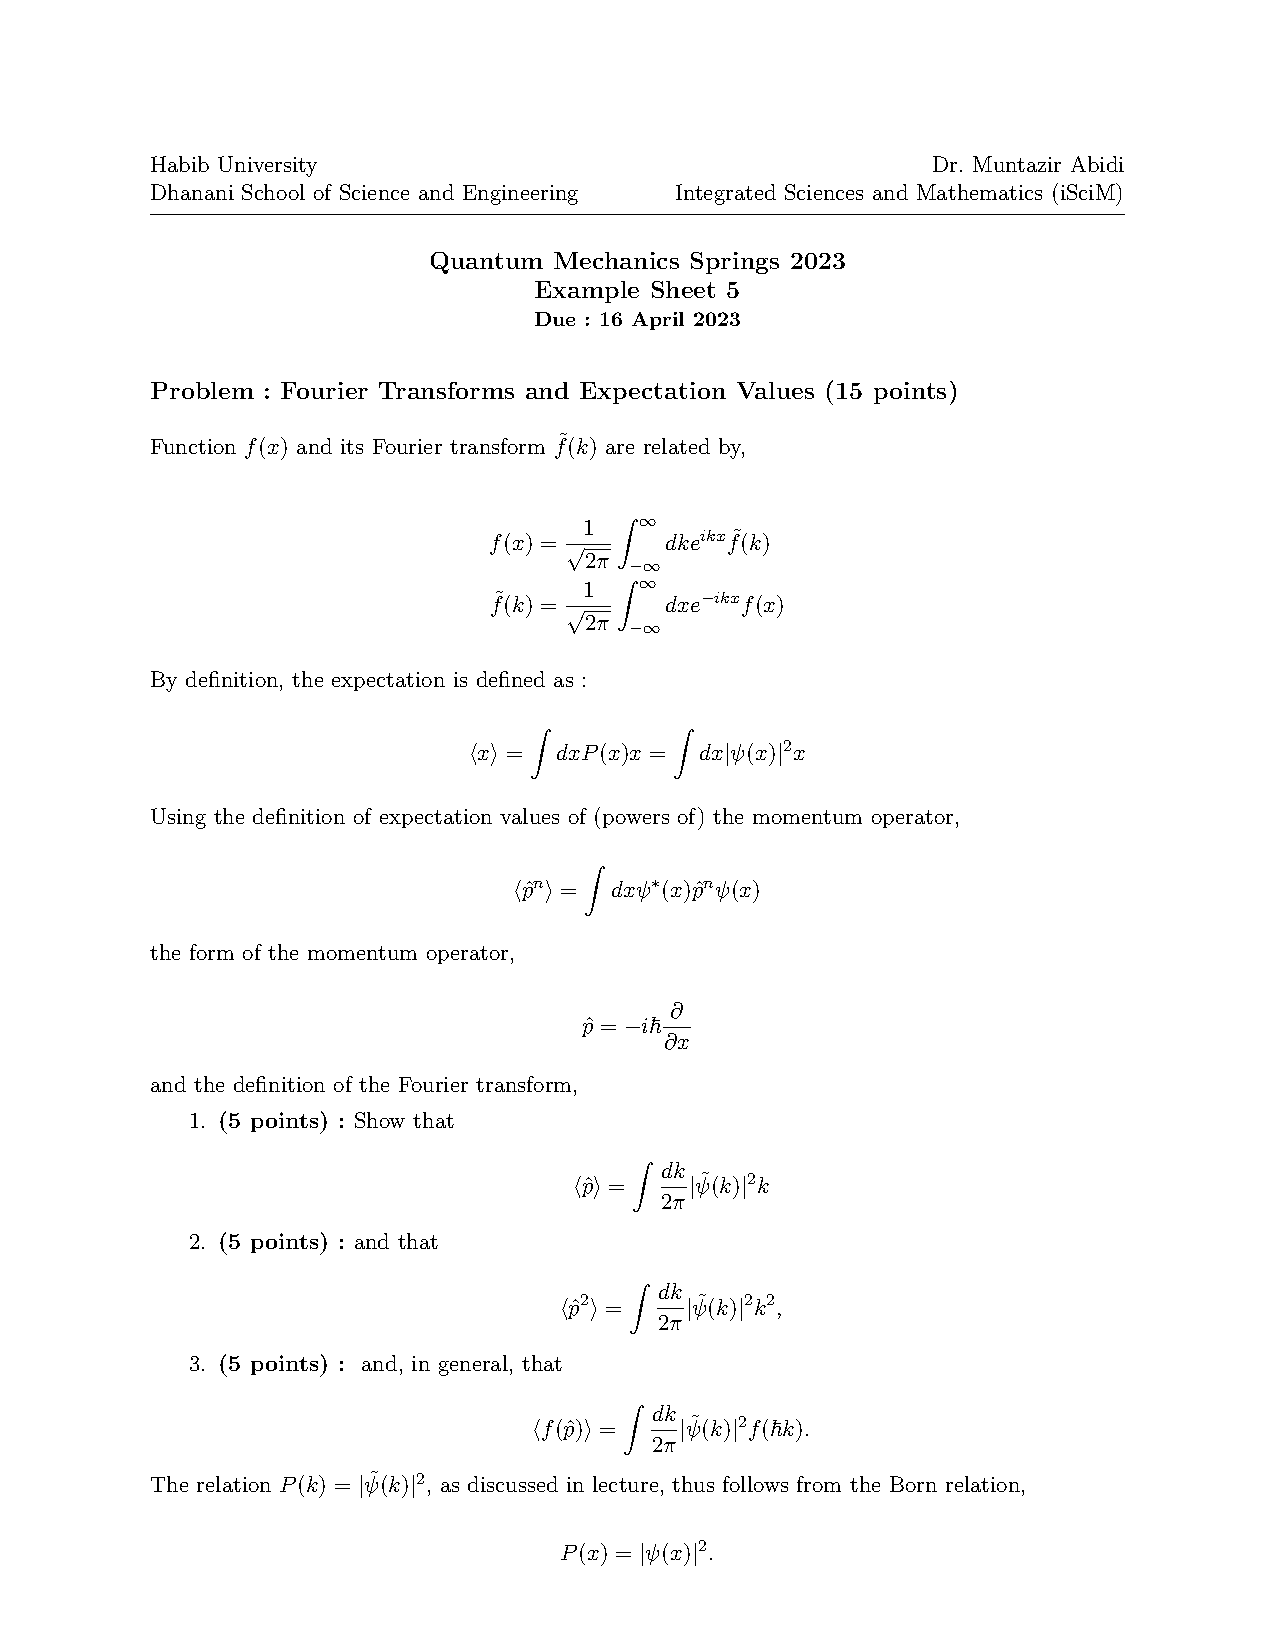
\includepdf[pages=-]{Assignment5_QM.pdf}
\end{document}
